\documentclass[mainlanguage=french,fncychap=none, secnumdepth=paragraph]{yathesis}

\DeclareUnicodeCharacter{0301}{\'{e}} 
% Chargement manuel de packages (pas déjà chargés par la classe yathesis)
\usepackage[T1]{fontenc}
\usepackage[utf8]{inputenc}
\usepackage{lipsum} % À proscrire dans un vrai mémoire de thèse !
\usepackage{hyperref}

\usepackage{booktabs} % pour des beaux tableaux
\usepackage{graphicx} % pour \inclugraphics
\usepackage{pgfplots} % pgfplots
\usepackage{amsmath,mathtools, amsfonts}
\usepackage{stmaryrd, bbold}
\usepackage{tcolorbox}
\usepackage{xcolor} % les couleurs
\usepackage{algorithmic,algorithm} % les algorithmes

\usepackage[utf8]{inputenc}
\usepackage[T1]{fontenc}
%\usepackage[Lenny]{fncychap}    changer forme chapitre

\usepackage{siunitx}

% yathesis configuration (choisissez votre labo !)
\apptocmd{\makebackcover}{\par\bigskip\centering
\includegraphics[width=1cm]{logos/ljll}}{}{}
%
\expression{aim}{En vue de l’obtention du grade de docteur de }{In order to become Doctor from }

%\apptocmd{\makebackcover}{\par\bigskip\centering
\includegraphics[width=1cm]{logos/lpsm}}{}{}
%
\expression{aim}{En vue de l’obtention du grade de docteur de }{In order to become Doctor from }

%\apptocmd{\makebackcover}{\par\bigskip\centering
\includegraphics[width=1cm]{logos/imj-prg}}{}{}
%
\expression{aim}{En vue de l’obtention du grade de docteur de }{In order to become Doctor from }

%\input{config/yathesis_ceremade}

% macros
% 
\newcommand\vect[1]{\bm{#1}}
\newcommand\conj[1]{\overline{#1}}

% derivées
\newcommand\der[2]{\dfrac{\mathrm{d} #1}{\mathrm{d} #2}}
\newcommand\derpart[2]{\dfrac{\partial #1}{\partial #2}}

% maths
\newcommand\R{\mathbb{R}}
\newcommand\Z{\mathbb{Z}}
\newcommand\I{\mathrm{i}}
\newcommand\E{\mathrm{e}}
\let\geq\geqslant
\let\leq\leqslant
\newcommand\D{\mathrm{d}}
\newcommand\norm[2]{\left\|#1\right\|^{#2}}
\newcommand\prodscal[2]{\langle#1,\;#2\rangle}
\newcommand\sphere{\mathbf{S}}
\DeclareMathOperator*{\argmax}{arg\,max}
\DeclareMathOperator*{\argmin}{arg\,min}

\newcommand{\ndr}[1]{\textcolor{blue}{[#1]}}

\newcommand{\p}{\partial}
\newcommand{\diff}{\,\mathrm{d}}
\newcommand{\RR}{\mathbb{R}}
\newcommand{\CC}{\mathbb{C}}
\newcommand{\PP}{\mathbb{P}}
\newcommand{\f}[2]{\frac{#1}{#2}}
\newcommand{\mellin}{\mathcal{M}}
\renewcommand*{\hat}{\widehat}
\newcommand{\iid}{\textit{i.i.d.}\;}

% style
\newcommand\latin[1]{\textit{#1}}
\newcommand\imp[1]{\textcolor{red!70}{#1}}

% intervalle d'entier
\newcommand\interint[2]{\left\llbracket 1, 5\right\rrbracket}

% Remark
\newenvironment{Remark}{%
\tcbset{%
arc=0pt,outer arc=0pt,colback=gray!10!white,colframe=gray!60!white,
boxsep=0pt,left=5pt,right=5pt,top=8pt,bottom=8pt, bottomtitle = 3pt, toptitle=3pt,
boxrule=0pt,bottomrule=0.5pt,toprule=0.5pt}
\begin{tcolorbox}[fonttitle=\sffamily\bfseries,title=Remark]}%
{\end{tcolorbox}}

%% les couleurs/ colors
\definecolor{theoreme}{RGB}{8,8,88}
\definecolor{definition}{RGB}{88,8,8}
\definecolor{tableau}{RGB}{232,208,157}
\definecolor{preuve}{RGB}{8,88,8}
\definecolor{propriete}{RGB}{88,44,8}
\definecolor{fgris}{RGB}{160,160,160}
\definecolor{matlab}{RGB}{52,73,112}
\definecolor{result}{RGB}{42,53,162}
\definecolor{darkred}{rgb}{.7,0,0}
\definecolor{linkColor}{rgb}{.7,0,0}
\definecolor{relief}{rgb}{.7,0,0}
% la bibliographie
\usepackage[backend=biber, maxbibnames=6, maxcitenames=6,
mincitenames=1, firstinits=true, doi=false,isbn=false,url=false]{biblatex}

\addbibresource{bibliographie.bib}

\begin{document}

% informations sur la these
\author[contact@guillaumegarnier.com]{Garnier}{Guillaume}
\title{Effets d'une mutation sur la valeur sélective d'une bactérie}
\subtitle{Estimation théorique et implémentation numérique}
\academicfield{Mathématiques appliquées}
\speciality{Statistiques}
\date{??}{??}{202?}
%\submissiondate{1}{10}{2014}
% (Facultatif) Sujet pour les méta-données du PDF :
\subject{Effets d'une mutation sur la valeur sélective d'une bactérie : Estimation théorique et implémentation numérique}

\supervisor[professor,affiliation=INRIA]{Marie}{Doumic}
\cosupervisor[mcf,affiliation=CEREMADE]{Marc}{Hoffmann}
\cosupervisor[mcf,affiliation=INRAE]{Lydia}{Robert}
\referee[professor,affiliation=IHP]{René}{Descartes}
\referee[seniorresearcher,affiliation=CNRS]{Denis}{Diderot}
\committeepresident[professor,affiliation=ENS Lyon]{Victor}{Hugo}
\examiner[mcf,affiliation=Université de Paris~13]{Sophie}{Germain}
\examiner[juniorresearcher,affiliation=INRIA]{Joseph}{Fourier}
\examiner[juniorresearcher*,affiliation=CNRS]{Paul}{Verlaine}

\keywords{Estimation nonparamétrique, Problèmes inverses}{Nonparametric statistics, Inverse Problems}


% informations dépendantes du labo (choisissez votre labo !)
\institute[logoheight=1.25cm,logo=logos/su,url=https://www.sorbonne-universite.fr/]{Sorbonne Université}
%
\company[logo=logos/LJLL,url=https://ljll.math.upmc.fr/]{LJLL}
%
\doctoralschool[url=http://www.ed386.upmc.fr/]{École Doctorale Sciences Mathématiques de Paris Centre}
\laboratory[
logo=logos/LJLL,
logoheight=3.25cm,
telephone= +33 1 44 27 42 98,
url=https://www.ljll.fr/
]{Laboratoire Jacques-Louis Lions}{%
  Sorbonne Université\\
  Campus Pierre et Marie Curie\\
  4 place Jussieu            \\
  75005 Paris                \\
  France}

%\institute[logoheight=1.25cm,logo=logos/su,url=https://www.sorbonne-universite.fr/]{Sorbonne Université}
%
\company[logo=logos/lpsm,url=http://lpsm.paris]{LPSM}
%
\doctoralschool[url=http://www.ed386.upmc.fr/]{École Doctorale Sciences Mathématiques de Paris Centre}
\laboratory[
logo=logos/lpsm,
logoheight=3.25cm,
telephone= +33 1 57 27 93 16,
url=https://www.lpsm.paris/
]{Laboratoire de Probabilités, Statistique et Modélisation}{%
  Sorbonne Université\\
  Campus Pierre et Marie Curie\\
  4 place Jussieu            \\
  75005 Paris                \\
  France}

%\institute[logoheight=1.25cm,logo=logos/su,url=https://www.sorbonne-universite.fr/]{Sorbonne Université}
%
\company[logo=logos/imj-prg,url=https://www.imj-prg.fr]{IMJ-PRG}
%
\doctoralschool[url=http://www.ed386.upmc.fr/]{École Doctorale Sciences Mathématiques de Paris Centre}
\laboratory[
logo=logos/imj-prg,
logoheight=3.25cm,
%telephone=,
url=https://www.imj-prg.f
]{Institut de Mathématiques de Jussieu-Paris Rive Gauche}{%
  Sorbonne Université\\
  Campus Pierre et Marie Curie\\
  4 place Jussieu            \\
  75005 Paris                \\
  France}

%\input{config/infos_ceremade}

\maketitle[frametitle=none]

\makekeywords

\makelaboratory

\dedication{À Manue}
\dedication{À Garance}
\dedication{À mes parents}
\dedication{À Grégoire}
%\makededications

% Épigraphes(s) :
%\frontepigraph{Il est plus facile de désintégrer un atome qu'un préjugé.}{Albert Einstein}
% Production de la page de d'épigraphe(s) :
%\makefrontepigraphs

\begin{abstract}
French version
\end{abstract}
\begin{abstract}
English version
\end{abstract}


\makeabstract

\tableofcontents

%\chapter{Remerciements}

Directeurs de thèses \par

Jury \par

La chaire MMB, L'Inria (peut-être l'ERC de Sylvie)

CEMRACS / Collaborateurice
(Olga, Joubine, Marie, Miguel)

Potes Orsay
Laboratoire

Sources d'inspirations : Prévert

Activité extra-scolaire : POFM, ETEAM, TFJM

Mention spéciales Charles, Margot, Claire, Nathanaël

Parents \par

Remercier Manue et affichier Mr. Navet et les Jellycats \par

Remercier Garance \par

Grégoire

Nounours, Kawacci, Hash, Rico, Sassy \& Aqua 



\mainmatter


Tous les organismes subissent des mutations. Une mutation est une altération spontanée ou provoquée du support de l'information génétique. C'est un mécanisme qui joue un rôle clé dans l'histoire de la vie; en particulier, il explique l'apparition de nouveaux caractères héréditaires au sein d'une population. \\
    
Ces nouveaux caractères peuvent modifier la \emph{valeur sélective} d'un individu. La valeur sélective, appelée aussi \emph{fitness}, est un concept fondamental en biologie évolutive. Introduit par Darwin en 1859 dans son ouvrage \textit{On the Origin of Species} \cite{darwin1859origin}, ce terme désigne la capacité d'un individu ayant un certain génome à survivre et à se reproduire.\\
    
    On distingue trois types de mutations : 
        \begin{itemize}
            \item Certaines sont délétères voir létales, c'est-à-dire qu'elles réduisent le développement de l'individu ou le tuent.
            \item Certaines sont neutres et n'induisent aucun effet sur le développement. 
            \item Certaines sont bénéfiques et favorisent le développement de l'individu.
        \end{itemize}
            
    Les effets d'une mutation sur la valeur sélective d'un individu sont plus ou moins marqués, ce qui forme ainsi un continuum d'effets. \\
    
    La manière dont ces mutations affectent la valeur sélective d'un individu est une question centrale en biologie évolutive. En particulier, les biologistes s'intéressent à la densité de la répartition de ces effets \emph{(DFE, Density Fitness Effect)}.\\
    
    Connaître la forme de la DFE est une question essentielle. Dans un article publié en 2007 \cite{eyre2007distribution}, Eyre-Walker et al. donnent plusieurs exemples dans le but d'insister sur l'importance de son étude.
        \begin{itemize}
            \item Dans l'espèce humaine, le génome d'un individu possède plus d'une centaine de nouvelles mutations que l'on ne retrouve pas chez ses parents. L'étude de la DFE permet d'étudier leurs effets afin de savoir s'ils sont bénéfiques ou non.
            \item La DFE permet de comprendre et de quantifier la diversité génétique que l'on retrouve dans les maladies humaines ainsi que son évolution future.
            \item La DFE permet de prévoir les conséquences du maintien à petite taille d'une population d'animaux ou de plantes, comme dans les programmes d'élevage en captivité. \\
        \end{itemize}
        
    L'étude de la DFE est un passage obligé pour comprendre et prévoir la trajectoire évolutive d'une population et répondre à plusieurs questions qui restent encore en suspens.\\
    
    Cependant, il est difficile d'obtenir une estimation de la DFE \cite{bataillon2014effects}. En particulier, jusqu'à présent les moyens techniques ne permettaient pas d'observer précisément l'apparition d'une mutation dans le génome. \\
    
    %Pour se rendre compte qu'une mutation était apparue, il était nécessaire de le déduire à partir d'une variation du phénotype. \\


    Le point de départ de ce projet est un article de 2018 écrit par Lydia Robert et al. \cite{robert2018mutation}. Dans cet article, les auteur.ices présentent un nouveau protocole expérimental qui permet de suivre en temps réel l'apparition de nouvelles mutations chez \textit{E. coli}. \\
    
    Cette nouvelle méthode expérimentale permet d'obtenir de nouvelles données  afin d'estimer la DFE. En effet, il est possible grâce à ces données de savoir immédiatement quand une mutation apparaît. D'autres expériences permettent de regarder l'évolution de la valeur sélective d'une cellule au cours du temps. \\
    
    Dès lors, plusieurs méthodes sont possibles pour tenter d'estimation de la DFE à partir de ces observations expérimentales. Cependant il s'agit d'un problème inverse sévèrement mal posé. \\
    
    Dans ce mémoire, nous proposons d’étudier une question particulière d’estimation: 
    
        \begin{center}
            \textit{Inférer la DFE à partir de mesures expérimentales de la valeur sélective au cours du temps au sein d'une lignée cellulaire.}
        \end{center}
        
    Pour répondre à cette question, nous devrons prendre en compte que les données expérimentales sont extrêmement  bruitées. 
    Cette question rejoint une problématique plus large qui a de nombreuses autres applications possibles. \\






\selectlanguage{english}

\chapter{Introduction}
    \input{chapters/chapitre1}
\section{Motivation}

\chapter{Description of the biological question}
    For over a century, researchers have tried to understand the impact of mutations on an individual's selective value. However, this understanding remained limited, in particular because experimental techniques did not allow the appearance of new mutations to be observed directly, or their effects to be measured precisely. 

In a 2018 article, Robert and al. \cite{robert2018mutation} propose to overcome this difficulty by describing a new experimental method that makes it possible to see the appearance of new mutations in real time. In the same article, they explain second experimental method for estimating the selective value of a cell line over time.
These new techniques provide new data for understanding more precisely the impact of mutations on an individual's selective value. \\

In this section, we present the experimental techniques presented in \cite{robert2018mutation} as well as the available data.

\section{Detect mutations : \emph{Mutation Visualisation experiment}}

    \subsection{The Mismatch Repair}
    
Deoxyribonucleic acid (DNA) is a double-helix molecule that carries genetic information. It is an extremely precise piece of machinery, which means that the slightest disturbance to one of its strands is likely to alter the behaviour, and therefore the ability, of the cell to survive. \\

To avoid such events, living cells have developed complex repair systems capable of recognising and correcting these disturbances. When these systems correctly eliminate the disturbance, there are no consequences for the cell. On the other hand, when the repair system fails to eliminate the disturbance, a mutation occurs. \\

\subsubsection{DNA replication} During DNA replication, the two strands are separated by an enzyme: \emph{DNA Polymerase}. These strands (matrices) enable two new identical DNA helices to be reconstructed by base complementarity. The new strand is determined by the old strand: an A base on the mother strand will ensure a T base on the new strand, etc. (Figure \ref{fig:replication_adn}).

\begin{figure}
    \centering
    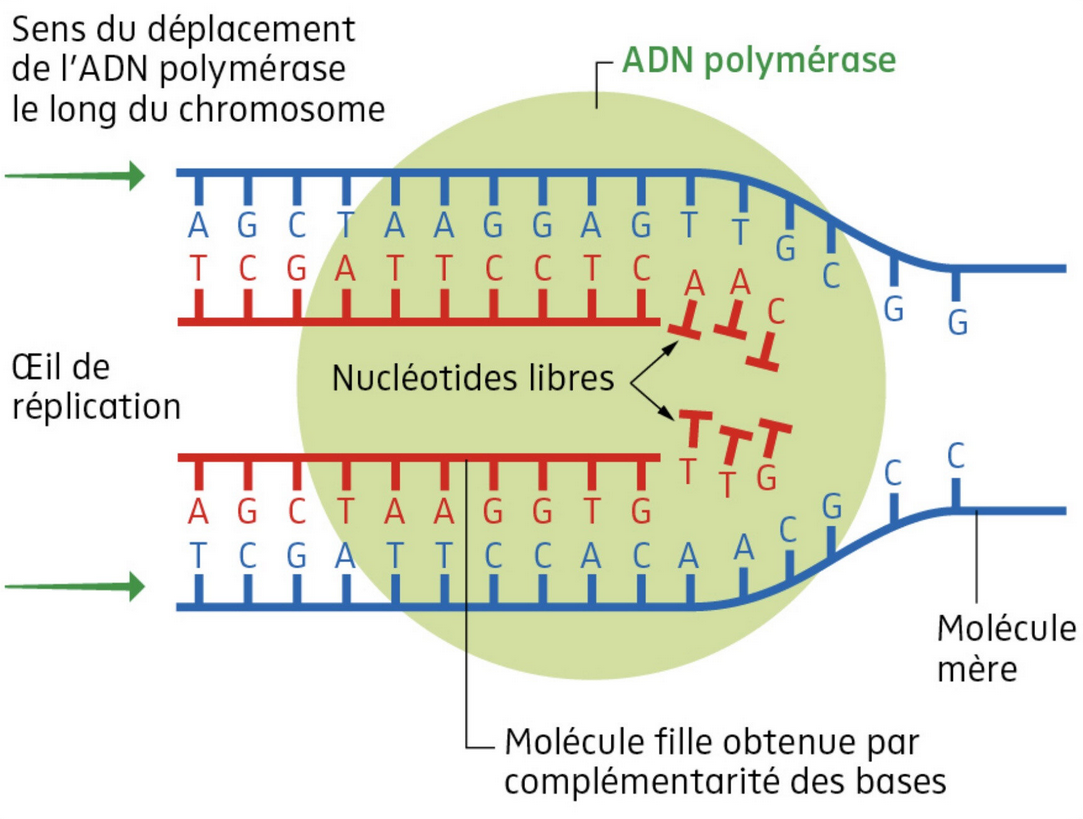
\includegraphics[width=0.5\textwidth]{pictures/replication_ADN.png}
    \caption{Simplified representation of a replication fork. Note that the new strands are complementary to the old strands. \\
     \ndr{Faire une image en anglais}}
    \label{fig:replication_adn}
\end{figure}

Sometimes a replication error occurs. In this case, one of the bases of the new strand is not complementary to its associated base. This is known as a mismatch. (Figure \ref{fig:mesappariement}).

\begin{figure}
    \centering
    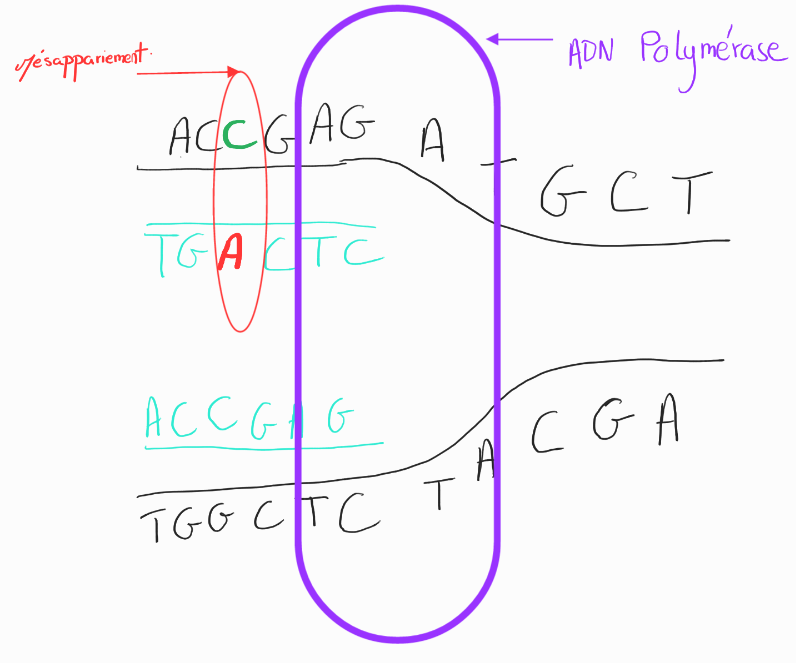
\includegraphics[width=0.5\textwidth]{pictures/mesappariement_adn.png}
    \caption{Artistic representation of a mismatch. A base G has been transformed into a base A.}
    \label{fig:mesappariement}
\end{figure}

\subsubsection{Mismatch detection and repair} 
The DNA Mismatch repair (MMR) is monitoring mechanism used during replication \cite{iyer2006dna}. It detects and repairs mismatches committed by the DNA polymerase during the replication process. The MMR system best known today is that of Escherichia coli, known as the MutHLS system, comprising the MutH, MutL and MutS proteins. \\

The repair system. The MutS protein recognises the mismatch and the MutL protein confirms the mismatch, then both bind to the DNA. The accumulation of MutS and MutL proteins activates the MutH protein, which cuts the neosynthesised strand. Resynthesis is then possible. (Figure \ref{fig:syst_mutHLS})

\begin{figure}
    \centering
    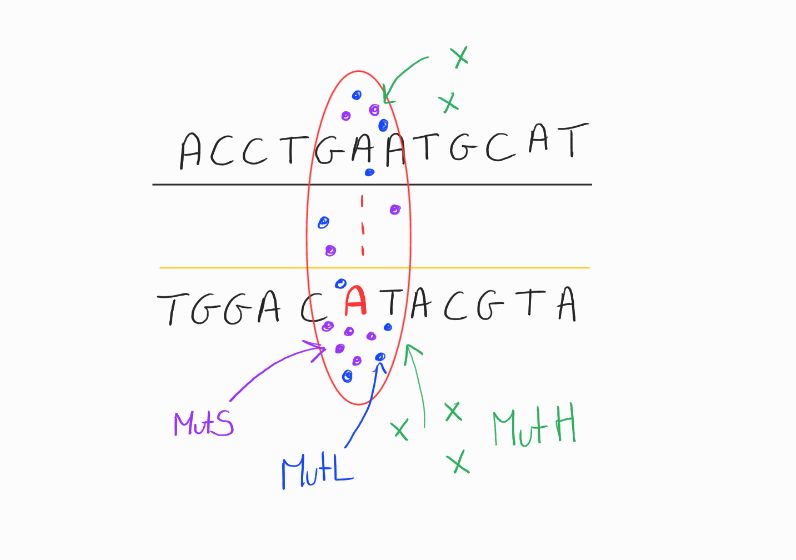
\includegraphics[width=0.8\textwidth]{pictures/syst_MutHLS.png}
    \caption{Schematic representation of the action of the mutHLS system.}
    \label{fig:syst_mutHLS}
\end{figure}


\subsubsection{The emergence of a mutation}

A mutation occurs when the mismatch repair system fails to repair a mismatch. In this case, the newly formed DNA has two mismatched bases. During replication, the DNA polymerase will form two new strands, one of which will carry a mutation compared to the original genome.
    
    \subsection{Real-time mutation detection}
    
    In \cite{robert2018mutation}, the authors develop a new strategy to observe the appearance of new mutations in real time. \\
    To begin with, they add a fluorescent protein (YFP) to the MutL protein. As the MutL proteins accumulate around the mismatch sites, it is possible to see the appearance of a new mutation using imaging techniques. \\
    In addition, the MutH endonuclease is deactivated to ensure that the mismatch is not repaired (Figure \ref{fig:syst_mutHLSmodifie}).

\begin{figure}
    \centering
    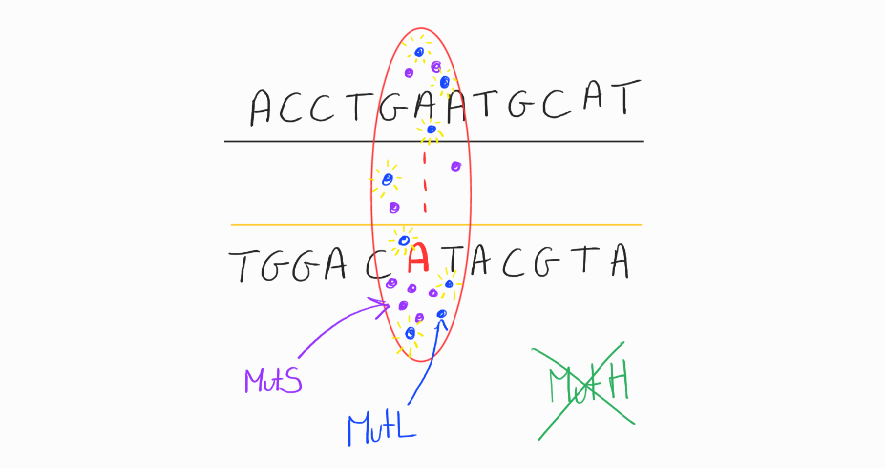
\includegraphics[width=0.8\textwidth]{pictures/syst_MutHLSmodifie.png}
    \caption{Schematic representation of the MV experiment}
    \label{fig:syst_mutHLSmodifie}
\end{figure}

\subsection{Discussion}

Using the results obtained in \cite{robert2018mutation}, the authors argue that the emergence of new mutations follows a Poisson process. 

\section{Measuring fitness: \emph{microfluidic Mutation Accumulation ($\mu$MA) experiment}} 

Mutation accumulation (MA) is the classic method for directly studying the effects of mutation \cite{mukai1964genetic,halligan2009spontaneous}. Several colonies of cells are derived from a single common ancestor. When the colonies have reached a sufficient size, a cell is randomly drawn from each colony to form a new one. \ndr{Mettre une figure}.
Several studies combine MA experiments with genome sequencing to estimate the rate and effects of mutations \cite{lynch2016genetic,tenaillon2016tempo} and MA experiment has been used to study mutations for several species \cite{katju2019old,ossowski2010rate,rutter2012fitness, baer2005comparative}. It is commonly assume that natural selection have no role in the evolution of colonies even if this method produces several selection biases that can skew the results \cite{mahilkar2022selection}. 

Microfluidic methods can be used to avoid these biases. The Microfluidic Mutation Accumulation ($\mu$MA) experiment is a technique developped in \cite{robert2018mutation,robert2019real} to study mutation rates, evolutionary dynamics and genetic stability in microorganisms. This experiment create a controlled environment where mutations can accumulate over successive generations without the selective pressures that typically eliminate deleterious mutations. By isolating and propagating single cells repeatedly, the µMA experiment allows to directly observe the effects of accumulated mutations on fitness, genome stability, and evolutionary trajectories, providing insights into how mutations contribute to genetic diversity and evolution. \\

In \cite{robert2018mutation}, the authors track the evolution of 1476 cell lines using microfluidic methods. For each new generation, only one daughter cell is kept, regardless of its fitness. \\
By filming the different cell lines over time, it is possible to measure changes in growth rates.

%\section{Description of the datasets}



\part{The theorical stuff}
\chapter{Statistical modelling}
    \section{Statistical approach method 1 - Decompounding noise}
    \section{Statistical approach method 2 - Multiplicative Decompounding}

\chapter{PDEs modelling}

\part{Data Analysis}
\chapter{Multimodality}
    Multimodality in a random sample refers to the presence of multiple local maxima or modes in the distribution of the sample data. Detecting multimodality is important because it suggests that the data might be better understood by considering multiple underlying groups or processes rather than a single, homogeneous population. For example, using a single mean to summarize a multimodal dataset might be misleading, as it does not capture the distinct groups within the data.

There is several reasons that may explain multimodality in a dataset. The following is a non-exhaustive list:
\begin{itemize}
    \item Identifying multimodality can lead to the discovery of subgroups with different characteristics. \ndr{citer source}
    \item Seasonality. \ndr{citer source}\\
\end{itemize}

In this chapter, we suppose that we observe a $n$-sample $(X_i, \, i=0\cdot n)$ assume to be \iid from an unknown probability density function $f$. We are interested in non-parametric tests which decide between the two hypothesis:
\begin{center}
    $H_0$ : $f$ is unimodal \qquad vs. \qquad  $H_1$ : $f$ is multimodal.
\end{center}
In Section~\ref{s:multimod_classic}, we present several classical tests for multimodality. In Section~\ref{s:multimod_application} we propose a procedure to detect multimodality with observations coming from compound poisson processes.

\section{Classical tests for multimodality}
\label{s:multimod_classic}

\subsection{The Silverman test}

\subsubsection{Presentation of the test}
The Silverman's test is a method commonly used to assess the number of modes or peaks in a density estimate \cite{silverman1981using,silverman1983some}. It is based on kernel estimators, due to Rosenblatt \cite{rosenblatt1956remarks} and Parzen \cite{parzen1962estimation}, which are classical estimators for approximating the probability density of a random variable whose $n$ sample $(X_i)$ \iid is observed. \\

The kernel estimator is defined as 
\begin{align*}
    \hat f_n(x, h) = \frac{1}{nh}\sum_{i = 1}^n K \Big( \frac{x-X_i}{h}\Big)
\end{align*}
where $K(u) = \frac{1}{\sqrt{2\pi}}\exp(-\frac{1}{2} u^2)$ and $h \in (0, \infty)$. \\

The choice of $h$ is a difficult one and must be made by the statistician. The number of modes of the estimator $\hat f_n$ depends on the size of $h$. If $h$ is very large, then the estimator has only one mode, whereas when $h$ is too small, we get a very spiky and over-fit estimate of the PDF. (See Fig~\ref{fig:choice_h}) \\


\begin{figure}[h]
    \centering
    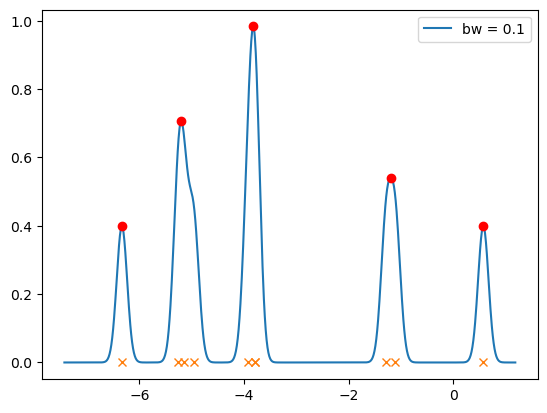
\includegraphics[width=0.27\paperwidth]{pictures/kernel_estim_over.png}
    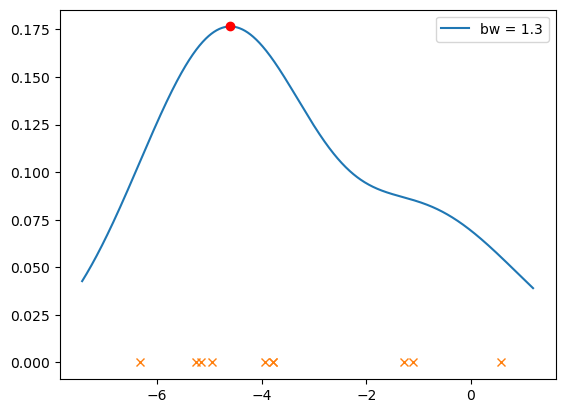
\includegraphics[width=0.27\paperwidth]{pictures/kernel_estim_under.png}
    \caption{(Left): $h$ is to small (Right): $h$ is to large}
    \label{fig:choice_h}
\end{figure}



In his paper , Silverman proves that using a Gaussian kernel ensures that decreasing $h$ will only introduce new local maxima \cite{silverman1981using}. Consequently, it is possible to find the minimum width $h_k$ such that $ \hat f_n(\cdot, h_k)$ has at most $k$ maxima for any integer $k \in \{1, \cdots, n\}$. \\

The estimator $\hat f_n(\cdot, h_k)$ form a family of kernel estimators, each with at most $k$ modes. In his paper, Silverman proposes a procedure for determining the significance of each of them. 

To do this, he uses a bootstrap method. The principle consists to evaluate the accuracy of the estimator by computing it on observations that are resampled from the original set of observations. \\

\textit{Methodology to evaluate the accuracy of the estimator} $\hat f(\cdot, h_k)$
\begin{enumerate}
    \item  First, draw a $n$-sample $X_{I(i)}$ with replacement from the the original set of observations
    \item Add some noise
    \begin{align*}
        y_i = \frac{1}{1+h_k^2/\sigma^2}(X_I(i) + h_k \varepsilon_i)
    \end{align*}
    where $\sigma$ is the standard deviation of $X_1, \ldots, X_n$, $h_k$ is the critical width we are testing, and $\varepsilon_i$ is a random value sampled from a normal distribution with mean 0 and standard deviation 1.
    \item Compute $\hat f_n(\cdot, h_k)$ for sample $y_i$. Check if $\hat f_n(\cdot, h_k)$ has less than $k$--mode. 
    \item Repeat. By repeating this operation several times, we calculate the $p$-value as the fraction of simulations where we did not find more than k modes.
\end{enumerate}


\subsubsection{Numerical examples}

\paragraph{A Gaussian mixture with 2 modes.} We illustrate the Silverman's test on the Gaussian mixture $0.6\mathcal{N}(-5,1)+0.4\mathcal{N}(0,1)$.
\begin{table}
\centering
\begin{tabular}{c|c|l}
Null hypothesis & p--value & bandwitdh \\
\hline
Reject 1 mode & p-value 0.99  & $h_1$ \, 1.3595962524414062 \\
Reject 2 mode & p-value 0.48  & $h_2$ \, 0.35981178283691406 \\
Reject 3 mode & p-value 0.75  & $h_3$ \, 0.33596038818359375 \\
Reject 4 mode & p-value 0.45  & $h_4$ \, 0.24213790893554688 \\
\end{tabular}
\caption{Result of the Silverman test for the Gaussian mixture with 2 modes}
\label{tab:silver_gm_2mod}
\end{table}
In Tab~\ref{tab:silver_gm_2mod}, we see that the null hypothesis : \textit{The density is unimodal} can be rejected with a $p$--value of 0.99. 

\subsection{The DIP test}

The DIP test, also known as the Hartigan's Dip Test, is a statistical test used to assess the unimodality of a data distribution. It measures the departure of the empirical distribution function of a sample from a unimodal distribution. Specifically, the test computes the maximum difference (or "dip") between the empirical distribution and the best-fitting unimodal distribution (defined as the least convex majorant and greatest convex minorant of the empirical distribution). A significant dip value indicates that the sample is not unimodal, suggesting the presence of multiple modes.

A unimodal distribution will have a Probability Density Function (PDF) that increases from 0 to some peak value and then decrease back to 0. When the PDF reaches a local maximum, then the Cumulative Distribution Function (CDF) switches from convex to concave.
A multimodal distributions CDF will change from convex to concave several times.\\

The concept behind the dip statistic is to gauge the extent of adjustment required for the cumulative distribution function (CDF) to become unimodal. Specifically, it represents the greatest distance, observed at any point, between the CDF and the nearest multimodal CDF. To put it differently, we can transform the distribution into a unimodal form by shifting the CDF by no more than the dip value at each instance. Essentially, the dip corresponds to the minimum value needed to achieve this transformation throughout the distribution.



\subsection{The Excess mass test}

\subsubsection{Presentation of the test}
The Excess Mass test is a statistical method used to assess multimodality in a data distribution by comparing the amount of probability mass concentrated in potential modes to what would be expected under unimodality.  It has been introduced by Müller and Sawitzki in 1991 \cite{muller1991excess}. The test evaluates the presence of multiple peaks by measuring the "excess mass," which refers to the extra density that appears around modes beyond what would be expected if the distribution were unimodal.

The Excess Mass test works by identifying regions in the data with significant density peaks and then calculating the total probability mass within these regions. This excess mass is compared to a reference unimodal distribution through optimization, which seeks to maximize the difference between observed density peaks and the unimodal fit. A significant excess mass indicates that the distribution has more than one mode.

The test is flexible and can be adjusted for different modes' widths and shapes, making it suitable for detecting multimodality in complex or irregular distributions. It is particularly useful in settings where traditional methods, like kernel density estimation, might struggle to identify multimodal structures. The results are typically interpreted through p-values or other statistical measures derived from comparisons with reference distributions generated via simulation or other means.\\


The empirical excess mass for $k$ modes and a constant $\lambda$ is defined as
\begin{align*}
    E_{n,k}(\PP, \lambda) = \sup_{C_1(\lambda), \ldots, C_k(\lambda)}
    \left\{
    \sum_{m = 1}^k \PP_n(C_m(\lambda))-\lambda\| C_m(\lambda)\|
    \right\}
\end{align*}
where the supremum is taken over all families $\{ C_m(\lambda) : m = 1, \ldots, l\}$ of closed intervals with endpoints at data points. $\|C_m\|$ denotes the measure of $C_m(\lambda)$ and 
\begin{align*}
    \PP_n(C_m(\lambda)) 
    = \frac{1}{n}\sum_{i = 1}^n
    \mathbb{1}_{X_i \in C_m(\lambda)}
\end{align*}

The key idea is that the difference $D_{n, k+1}(\lambda) = E_{n,k+1}(\PP, \lambda) - E_{n,k}(\PP, \lambda)$ represents the plausibility of the null hypothesis. The larger $D_{n, k+1}(\lambda)$ is, the more likely we are to reject $H_0$. \\

The excess mass statistic is defined as 
\begin{align*}
    \Delta_{n, k+1} = \max_{\lambda}\{D_{n, k+1}(\lambda)\}
\end{align*}

\subsubsection{Numerical examples}

\section{An application to the biological problem}
In this section, we apply 
\label{s:multimod_application}
\subsection{Simulation without noise}
\subsection{Simulation with noise}
\subsection{Real dataset}
%\section{The moment problem}

\appendix
\part{Appendix}
\chapter{Mathematic Tools}
\section{Nonparametric estimation}
\section{Statistical tests}
\section{Integral transformations}

\backmatter

\printbibliography

\makebackcover

\end{document}
%%% Local Variables:
%%% flyspell-mode: 1
%%% ispell-local-dictionary: "french"
%%% End:
